\section{Konzept\hfill\textnormal{\emph{Löbel}}}
Anschließend wurden über die objektorientierte Analyse die benötigten Klassen und Attribute definiert. 

\subsection{Technische Systemarchitektur}
Das technische System besteht aus folgenden Komponenten: Die Sensorik, die für das Senden und Empfangen von Signalen verantwortlich ist. Hier zählen unter anderem die Antennen zum Empfangen von Radiosignalen dazu. Ein LIDAR Sensor, über den Laserimpulse gesendet und reflektiertes gestreutes Licht bei Objekterkennung empfangen wird. Ein Wassersensor zur Messung der Kapazität, ob der Roboter sich an Land oder Wasser befindet (FR7) und ein Kraft- und Druckaufnehmer zur Gewichtsmessung der zu bergenden Gegenständen gehören auch dazu. Die Signalberechnung bzw. -wertung wird durch einen Microcontroller übernommen. Je nach empfangenen Signalwert werden die jeweiligen Motoren des Roboters gesteuert. Es werden unter anderem Motoren für den Greifer und Greifarm benötigt, als auch für den Antrieb von Ketten, Turbine, Ruder, das Drehen und Schwenken der Peripherie oder auch für die ausfahrbaren Stützen und den verschließbaren Deckel der Bergungsbox. Hinzu kommt die Peripheriesteuerung für die Kommunikation, die sich aus den Objekten Kamera, Lautsprecher und Mikrophon zusammensetzt. 

\begin{figure}[H]
  \centering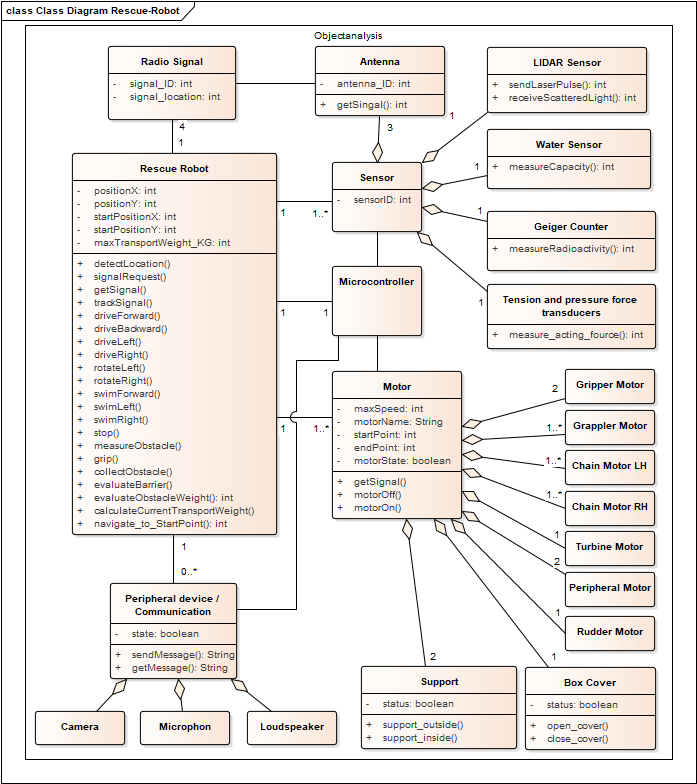
\includegraphics[width=1\linewidth]{Class Diagram Rescue-Robot.png}
  \caption{Class Diagram "Rescue Robot"}
  \label{ClassDiagram}
\end{figure}

\subsection{Subsysteme}
Nach Aufteilung der Objekte in die Kategorien "Signal transmit", "Signal reception“, "Signal calculation“, "Motor control“ und "Peripheral device control“ wurde eine Swimlane Analyse durchgeführt, in der der gesamte Prozessablauf beschrieben wurde. Daraus ergaben sich die folgenden Subsysteme: 

\begin{itemize}
\item das Firmengelände (siehe Abb. \ref{Systemumgebung})
\item die Signalverfolgung
\item die Fortbewegung (an Land und im Wasser)
\item die Objekterkennung (Hindernis, Person oder radioaktives Objekt)
\item die Navigation (Umfahren von Hindernissen)
\item die Kommunikation (zu Personen)
\item die Objektbergung (radioaktive Gegenstände)
\end{itemize}

Zu jedem dieser Subsysteme wurden detaillierte Aktivitätsdiagramme erstellt. Diese sind unter \textit{\url{https://github.com/BrunoBerger/Rescue-Robot.git}}im Ordner "Diagramme/Subsysteme/..." zu finden.\\ 
\\
Als erstes muss das \textit{Firmengelände} definiert sein, welches in Abschnitt \ref{map_} näher beschrieben wird. Die \textit{Fortbewegung} wird über die Ansteuerung der Motoren für Kettenantrieb (an Land) und Turbine und Ruder (im Wasser) realisiert (FR1 und FR2). Hierzu soll über den Wassersensor zunächst die Kapazität gemessen und bewertet werden. Gleichzeitig können über die Antennen am Rescue Robot Radiosignale empfangen werden. Die Radiosignale enthalten eine ID und auch einen Standort (x- und y-Koordinate) zum Berechnen der Distanz. In Abb.\ref{Track_Signal} wird die \textit{Signalverfolgung} beschrieben (FR6). Zur Signalverfolgung wird die Antenne genutzt, welche die kürzere Distanz zum Radiosignal bzw. Funkturm hat. Erst wenn die Radiosignal Distanz $<1$ ist, ist der jeweilige Funkturm erreicht.

\begin{figure}[H]
  \centering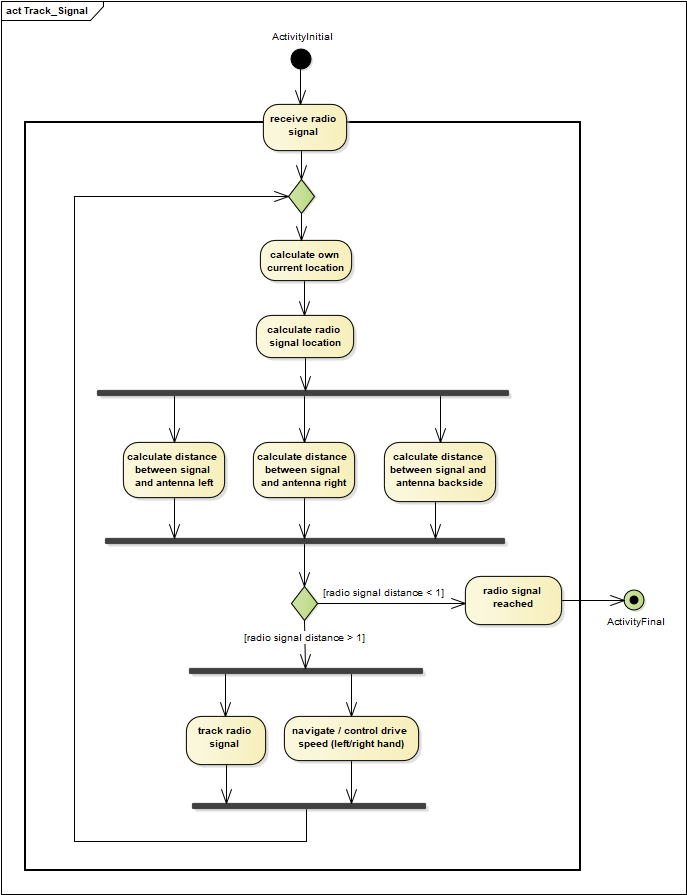
\includegraphics[width=1\linewidth]{Track_Signal.png}
  \caption{Subsystem: Aktivitätsdiagramm "Track Signal"}
  \label{Track_Signal}
\end{figure}

Zur \textit{Objekterkennung} soll der Rescue Robot nicht nur den LIDAR-Sensor nutzen, sondern parallel sollen zur Person-Erkennung auch die Kamera Bilder ausgewertet werden. Wenn eine Person erkannt wurde, soll die \textit{Kommunikation} gestartet werden. Dies passiert über Einschalten von Lautsprecher und Mikrophon. Der Rettungsdienst kann so mit der verletzten Person kommunizieren und über außen ggf. kleine "Erste Hilfe" leisten. Bei der \textit{Objektbergung} kommt es zu mehreren Schritten, siehe Abb.\ref{Rescue_object}. Wird ein Objekt erkannt, wird der Greifarm in die berechnete Position gefahren. Der Greifer öffnet sich und mittels Geiger Sensor wird die Radioaktivität des Objekts gemessen. Soll das Objekt aufgrund seines Strahlungswerts eingesammelt werden, schließt der Greifer sich. Gleichzeitig sind die Stützen des Rescue Robots ausgefahren. Nun wird der Greifarm angehoben und das Objektgewicht wird mittels Kraft- und Druckaufnehmer gemessen. Wird das maximale zulässige  Greif-Gewicht überschritten, öffnet der Greifer wieder und lässt das Objekt fallen. Ist das Objektgewicht im zulässigen Bereich, fährt der Greifarm die Position über der Box an, der Deckel wird geöffnet und das Objekt wird in die Box gelegt. Die funktionale Anforderung FR3 ist somit erfüllt. Anschließend wird das aktuelle Transportgewicht berechnet. Ist dies größer als das maximal zulässige Transportgewicht, soll der Rescue Robot wieder zurück zu seinem Startpunkt auf dem Firmengelände fahren, damit die Box geleert werden kann.

\begin{figure}[H]
  \centering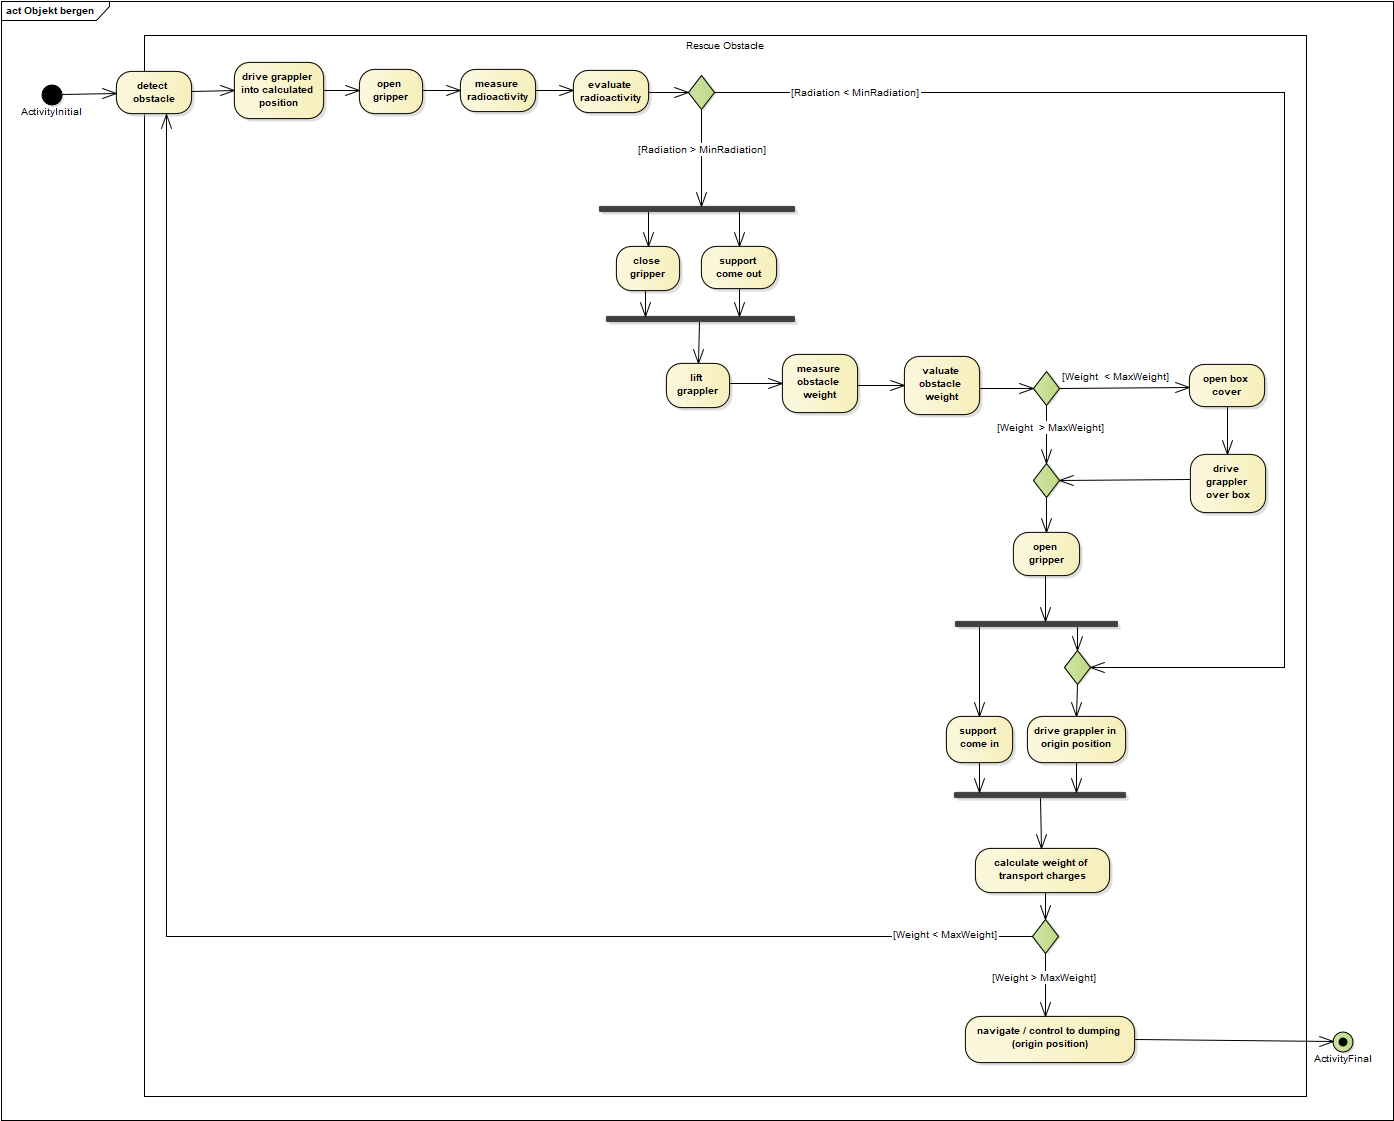
\includegraphics[width=1\linewidth]{Objekt bergen.png}
  \caption{Subsystem: Aktivitätsdiagramm "Rescue Object"}
  \label{Rescue_object}
\end{figure}